\documentclass[letter, 10pt]{article}
\usepackage{fullpage}
\usepackage[margin=0.5in]{geometry}
\usepackage{graphicx}
\usepackage{wrapfig}
\usepackage{caption}
\usepackage{subcaption}
\usepackage{listings}
\usepackage{hyperref}
\usepackage{amsmath}
\usepackage{float}

\pagenumbering{gobble}

\begin{document}
\noindent
\large \textbf{Rahul Ghosh} \hfill \textbf{Assignment\#2}\\
\normalsize Student ID: 5476965 \hfill CSci 5561\\

\section*{IMAGE REGISTRATION}
\subsection*{Methods}
Given an object/template, the aim of this project is to track the object/template in the given target frames as shown in Figure 1.

We begin by computing the sift features of both the template and target images using the $vl\_feat$ library and pruning those images using the ration test and bidirectional consistency. The matched features between the Template and Target1 are shown in Figure 2.

The images are now aligned using the features by calculating the transformation matrix A using RANSAC algorithm. The bounding box in Figure 3(a) shows the how the Template aligns with the Target Image. The target is then warped to the template image and the inital error image is shown in Figure 3(a). The transformation matrix is refined using the Inverse Compositional Image Alignment algorithm.

For multi-frame tracking we start with the original template and track it in Target1. We initialize the transformation matrix A using feature based image alignment. For every target iteration we use a initial A and refine it using inverse compositional alignment. Now we update the template by warping the target image and also update the initial A using the refined A for tracking in the next frame. Figure 3 shows the updating template image and the tracked object.

\subsection*{Results}
\begin{figure}[h]
    \minipage{0.49\textwidth}
        \centering
        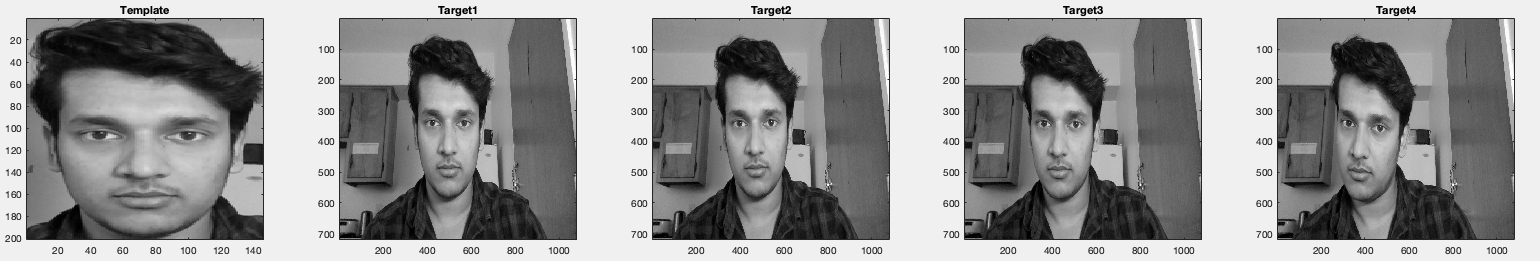
\includegraphics[width=\textwidth]{HW2/RESULT/FRAMES.png}
        \caption{Frames to track the object}
    \endminipage\hfill
    \minipage{0.49\textwidth}
        \centering
        \includegraphics[width=\textwidth]{HW2/RESULT/MATCHED_FEATURES.png}
        \caption{Matched Features}
    \endminipage\hfill
\end{figure}

\begin{figure}[h]
    \minipage{0.45\textwidth}
        \centering
        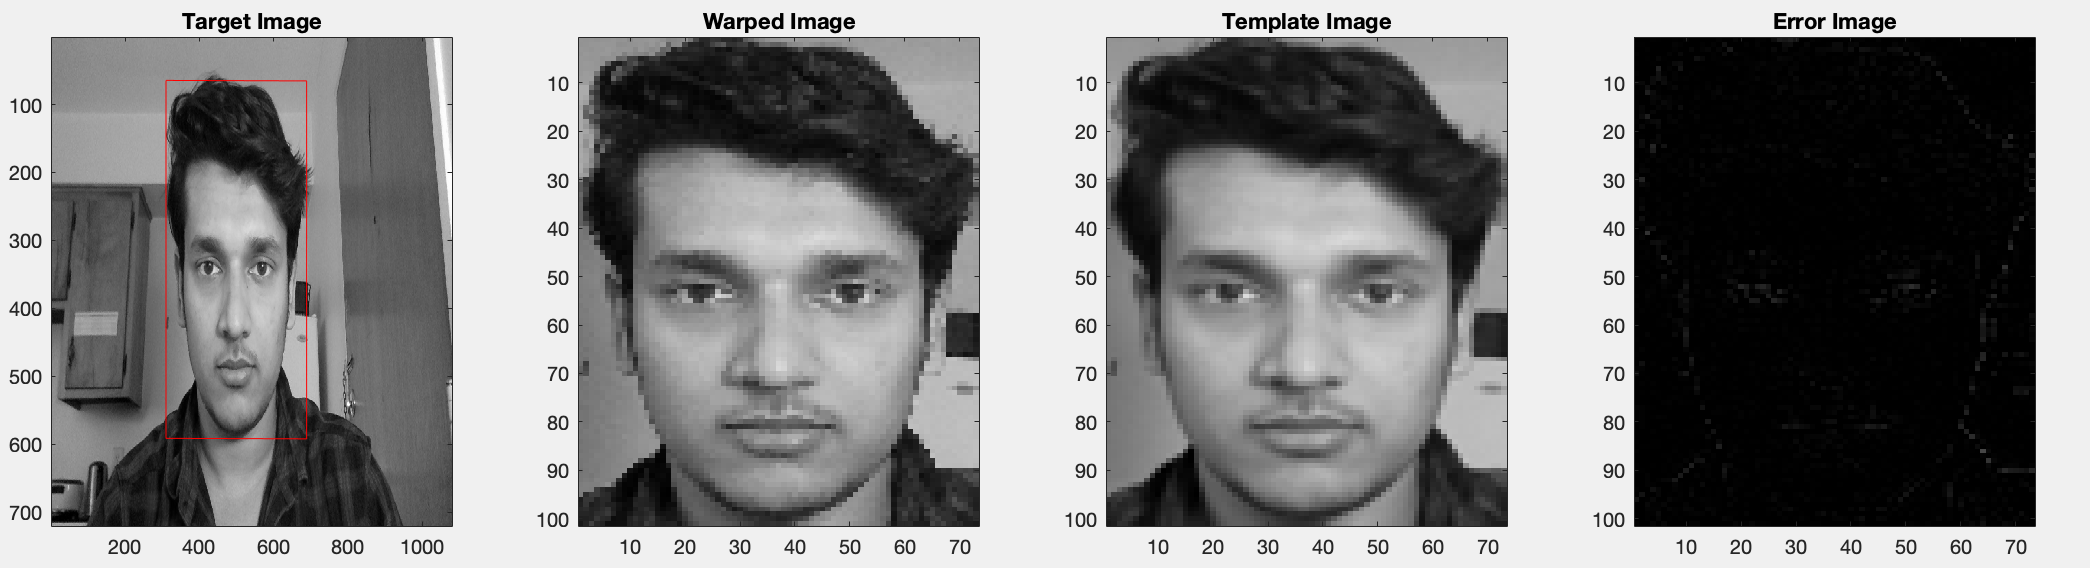
\includegraphics[width=\textwidth]{HW2/RESULT/FRAME1.png}
        \subcaption{Frame 1}
    \endminipage\hfill
    \minipage{0.45\textwidth}
        \centering
        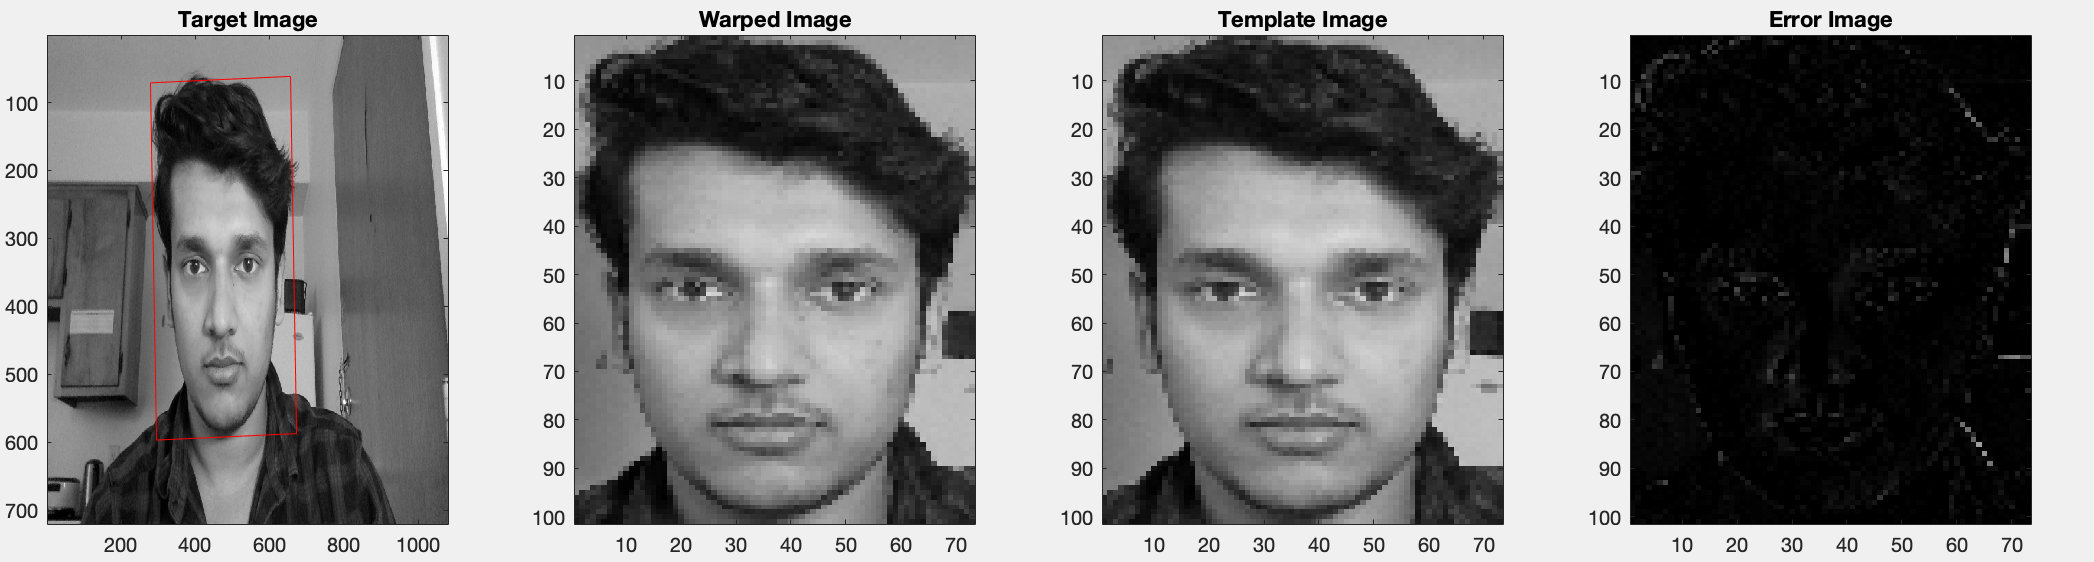
\includegraphics[width=\textwidth]{HW2/RESULT/FRAME2.png}
        \subcaption{Frame 2}
    \endminipage\hfill
    \minipage{0.45\textwidth}
        \centering
        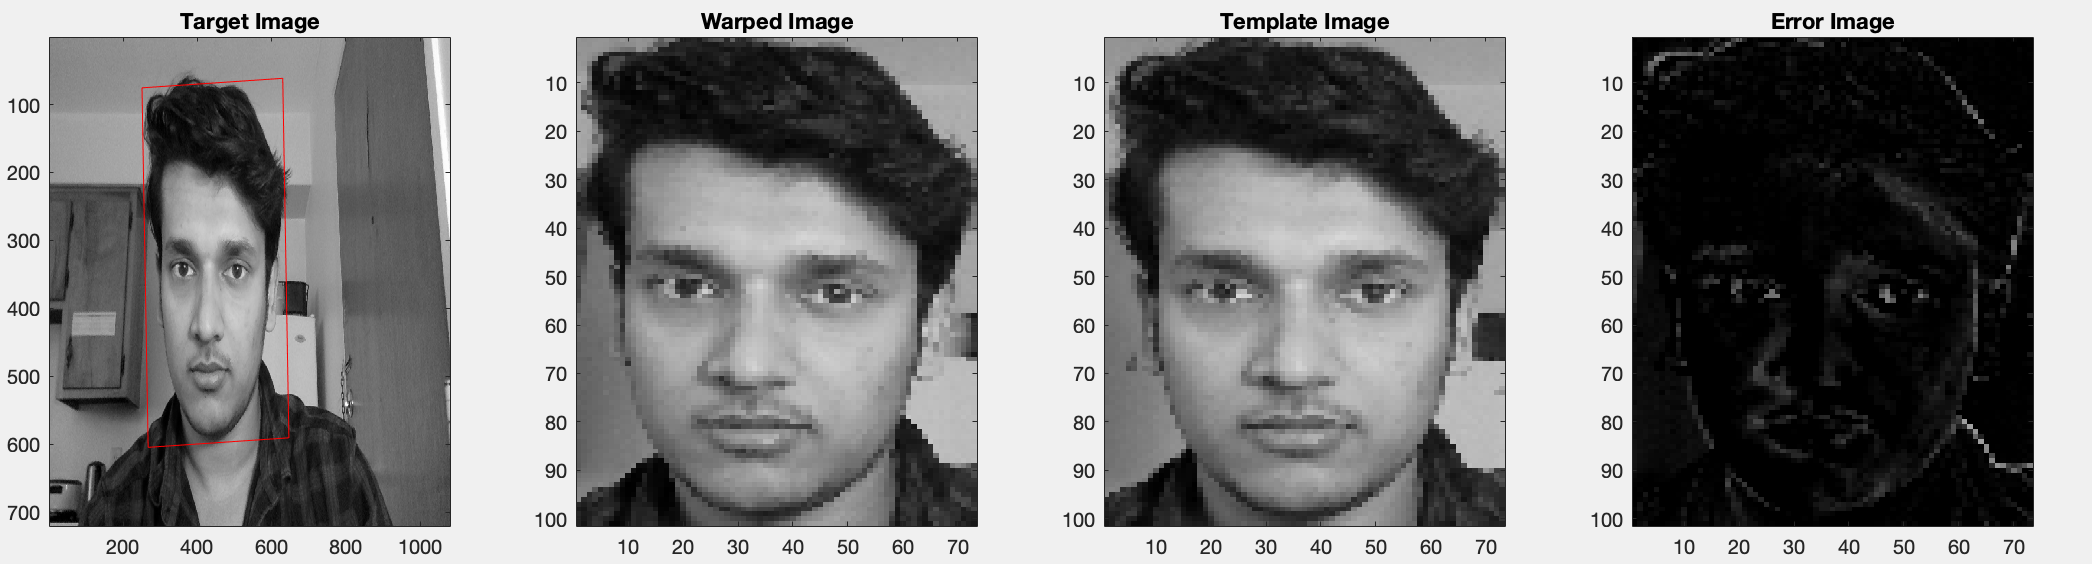
\includegraphics[width=\textwidth]{HW2/RESULT/FRAME3.png}
        \subcaption{Frame 3}
    \endminipage\hfill
    \minipage{0.45\textwidth}
        \centering
        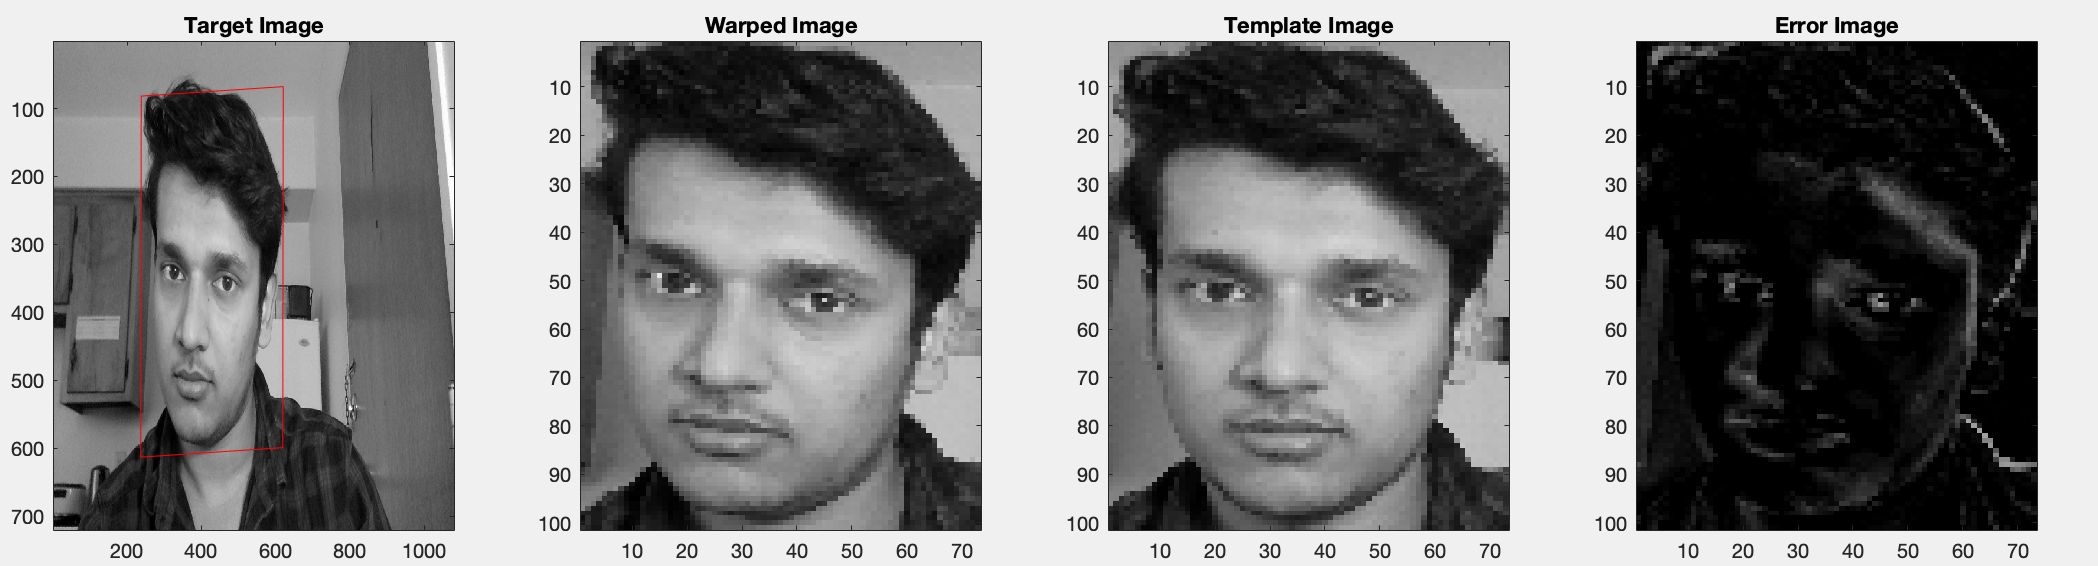
\includegraphics[width=\textwidth]{HW2/RESULT/FRAME4.png}
        \subcaption{Frame 4}
    \endminipage\hfill
    \caption{Multiframe Track}
\end{figure}

\end{document}